\documentclass{beamer}
\usepackage[utf8]{inputenc}
\usetheme{Warsaw}

\title{Comparing heuristics for the Steiner tree problem.}
\author{Antoine Huchet}
\date{\today}
%\institute{École Normale Supérieure, département de pipologie}

\begin{document}

\begin{frame}
\titlepage
\end{frame}

\begin{frame}
%MUTATION
	Mutation variation.
\begin{figure}
\centering
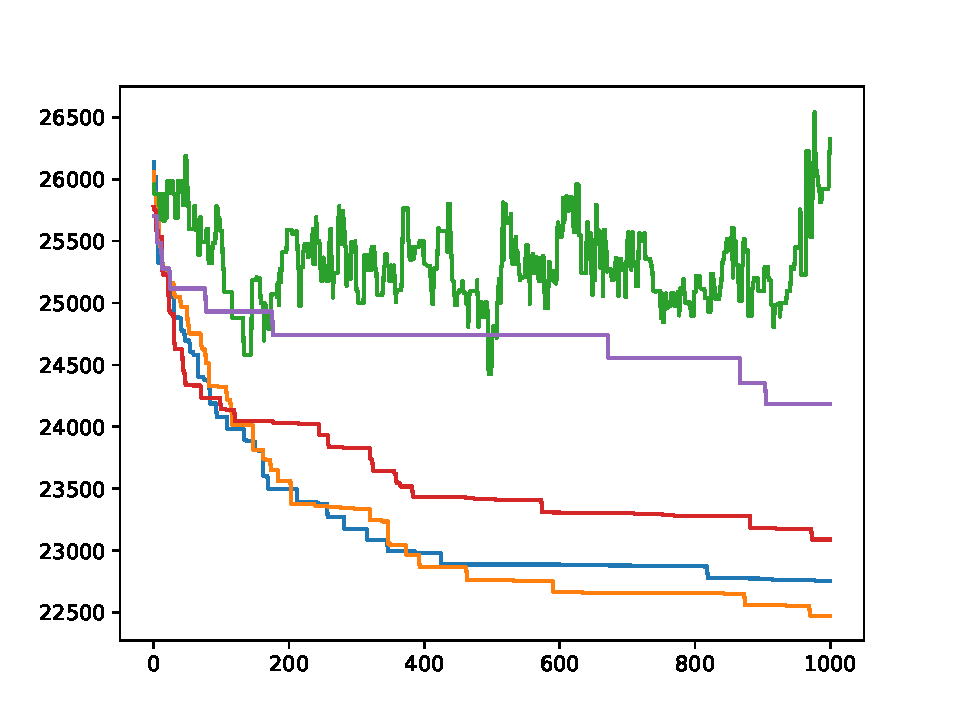
\includegraphics[scale=.5]{../Plots/new/5,2,mutation,eofb1000t-150.pdf}
\caption{Comparaison for $\lambda = 5$, $\mu = 2$ and mutation variation of
classic elitist selection (in blue), elitist selection on offsprings (in
orange), fitness proportional (in green), Boltzmann with constant $T = 1000$
(in red) and Threshold selection with constant parameter $T = -150$ (in
purple)}
\label{Mutationcompareselection}
\end{figure}
\end{frame}

\begin{frame}
	Crossover variation.
%CROSSOVER
\begin{figure}
\centering
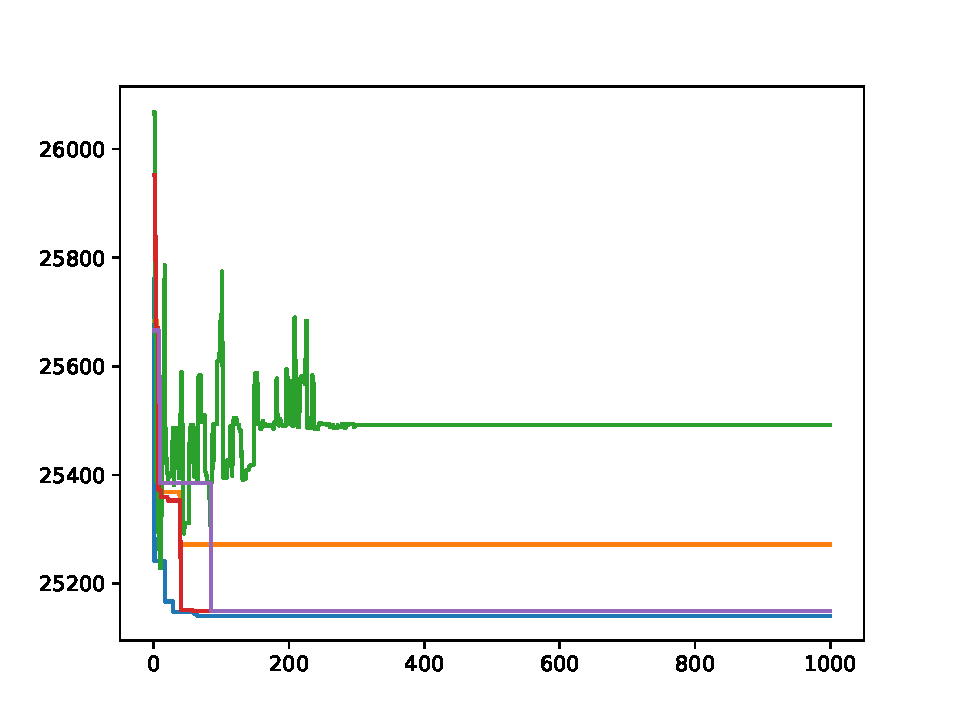
\includegraphics[scale=.5]{../Plots/new/5,2,crossover,eofb1000t-150.pdf}
\caption{Comparaison for $\lambda = 5$, $\mu = 2$ and crossover variation of
classic elitist selection (in blue), elitist selection on offsprings (in
orange), fitness proportional (in green), Boltzmann with constant $T = 1000$
(in red) and Threshold selection with constant parameter $T = -150$ (in
purple)}
\label{Crossovercompareselection}
\end{figure}
\end{frame}

\begin{frame}
	Both variations.
%MULTIPLE
\begin{figure}
\centering
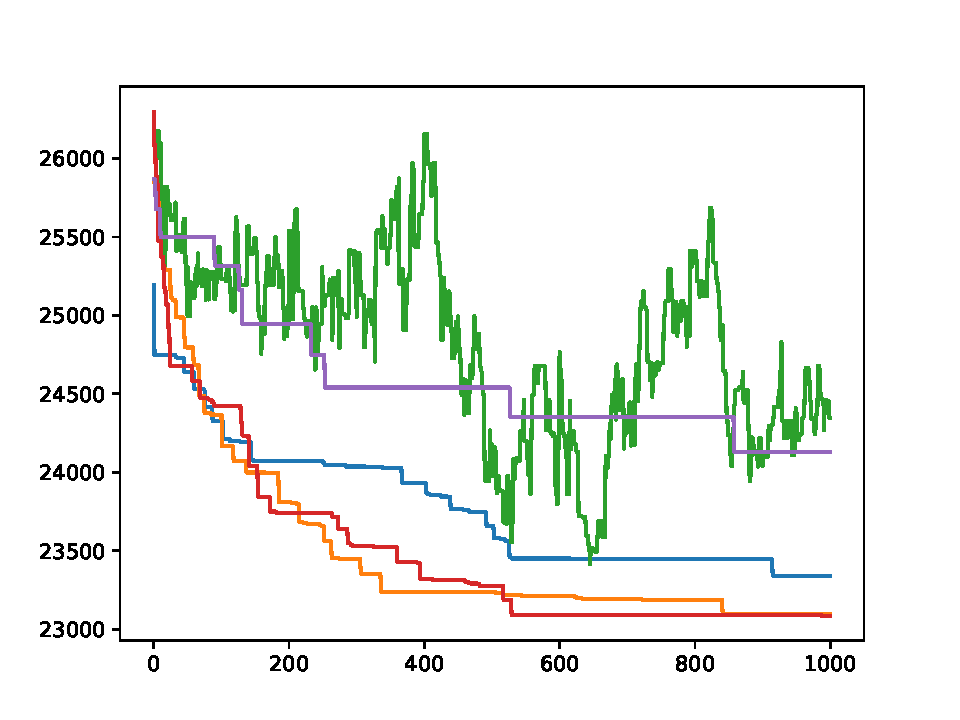
\includegraphics[scale=.5]{../Plots/new/5,2,multiple,eofb1000t-150.pdf}
\caption{Comparaison for $\lambda = 5$, $\mu = 2$ and multiple variation of
classic elitist selection (in blue), elitist selection on offsprings (in
orange), fitness proportional (in green), Boltzmann with constant $T = 1000$
(in red) and Threshold selection with constant parameter $T = -150$ (in
purple)}
\label{Multiplecompareselection}
\end{figure}
\end{frame}

\begin{frame}
	Elitist selection.
%ELITIST
\begin{figure}
\centering
%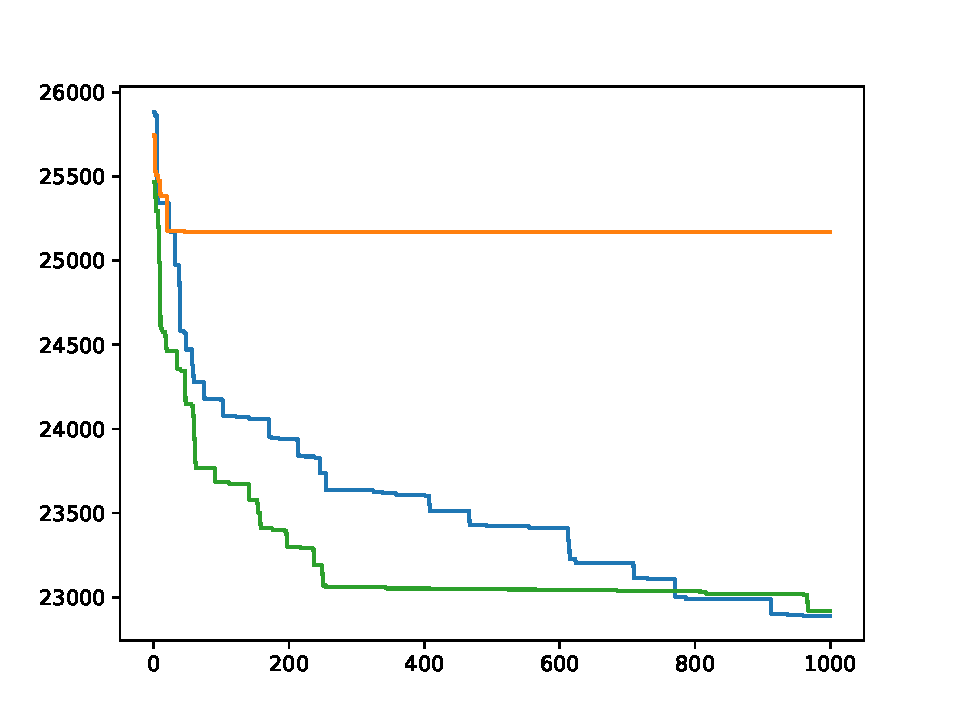
\includegraphics[scale=.5]{../Plots/5,2,elitist,mutcrossmult.pdf}
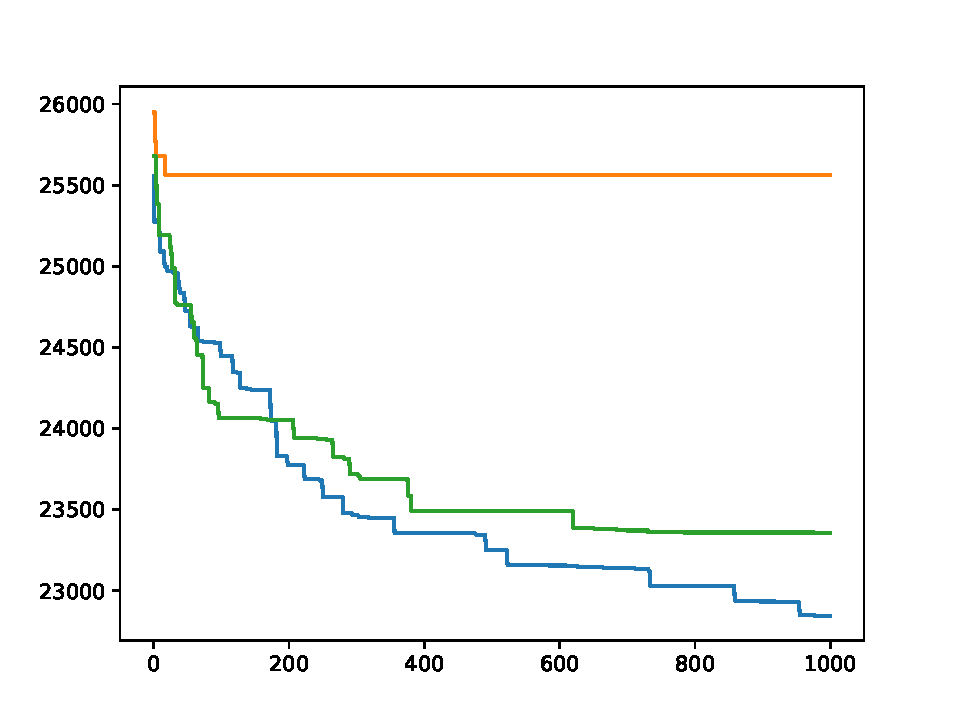
\includegraphics[scale=.5]{../Plots/new/5,2,mutcmul,elitist.pdf}
\caption{Comparaison for $\lambda = 5$, $\mu = 2$ and classic elitist selection
of mutation variation (in blue), crossover variation (in orange)  and another
variation consisting of a mix of both (in green).}
\label{Elitistcomparevariation}
\end{figure}
\end{frame}

\begin{frame}
	Elitist offsprings selection.
%OFFSPRINGS
\begin{figure}
\centering
%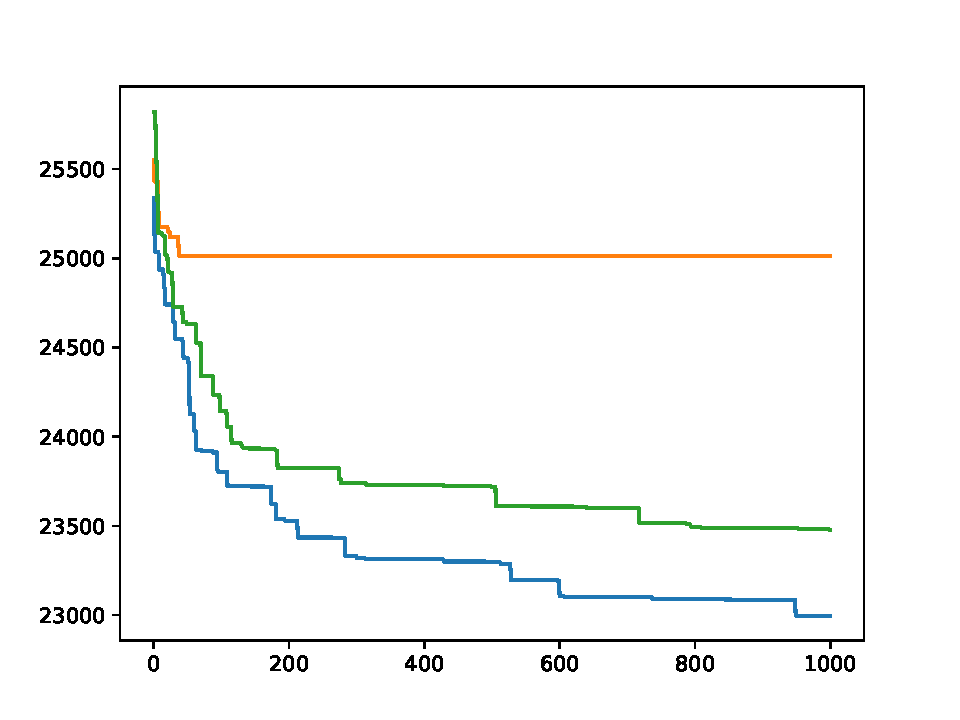
\includegraphics[scale=.5]{../Plots/5,2,offsprings,mutcrossmult.pdf}
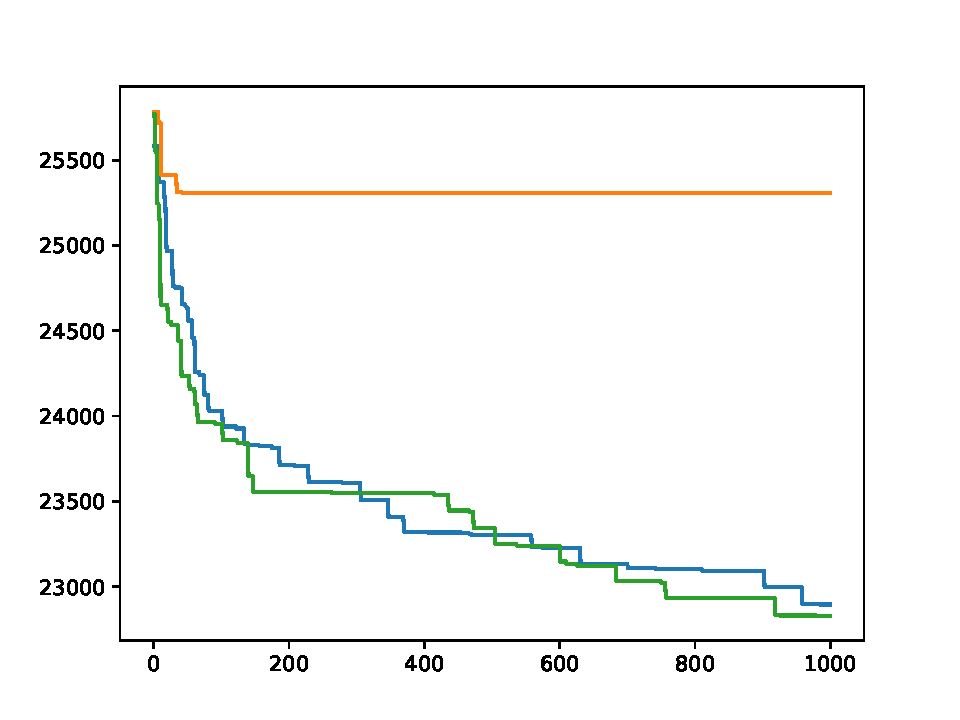
\includegraphics[scale=.5]{../Plots/new/5,2,mutcmul,offsprings.pdf}
\caption{Comparaison for $\lambda = 5$, $\mu = 2$ and offsprings elitist
selection of mutation variation (in blue), crossover variation (in orange)  and
another variation consisting of a mix of both (in green).}
\label{Offspringscomparevariation}
\end{figure}
\end{frame}

\begin{frame}
	Fitness selection.
%FITNESS
\begin{figure}
\centering
%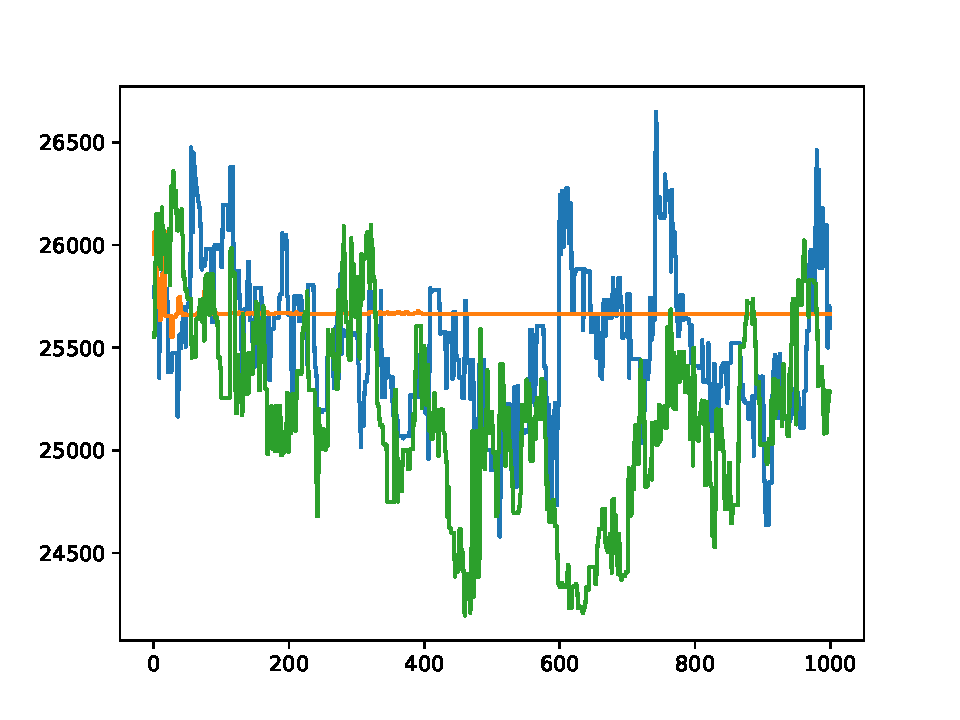
\includegraphics[scale=.5]{../Plots/5,2,fitness_prop,mutcrossmult.pdf}
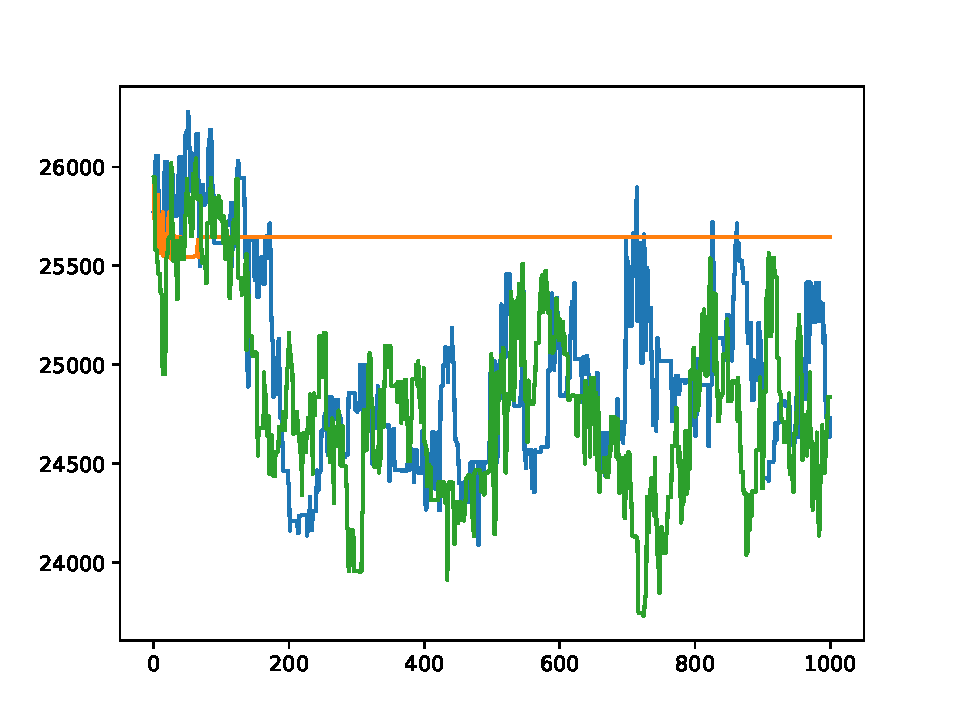
\includegraphics[scale=.5]{../Plots/new/5,2,mutcmul,fitness.pdf}
\caption{Comparaison for $\lambda = 5$, $\mu = 2$ and Fitness proportional
selection of mutation variation (in blue), crossover variation (in orange) and
another variation consisting of a mix of both (in green).}
\label{Fitnesscomparevariation}
\end{figure}
\end{frame}

\begin{frame}
	Boltzmann selection for constant $T = 1000$.
%BOLTZMANN
\begin{figure}
\centering
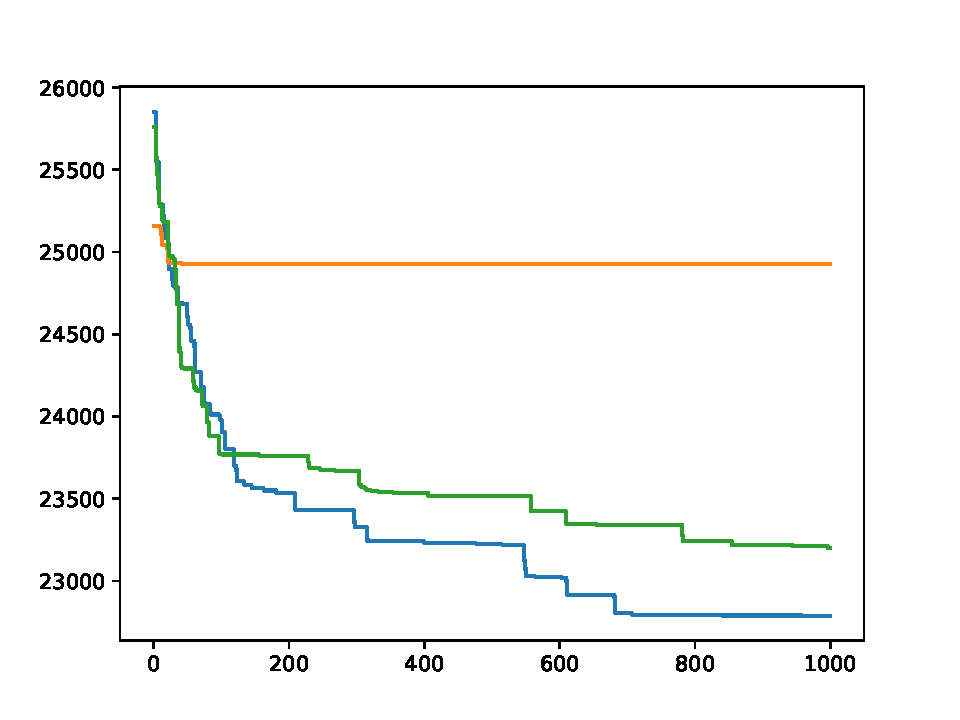
\includegraphics[scale=.5]{../Plots/new/5,2,mutcmul,Boltzmann1000.pdf}
\caption{Comparaison for $\lambda = 5$, $\mu = 2$ and Boltzmann selection with
constant parameter $T = 1000$ of mutation variation (in blue), crossover
variation (in orange) and another variation consisting of a mix of both (in
green).}
\label{Boltzmanncomparevariation}
\end{figure}
\end{frame}

\begin{frame}
	Threshold selection with $T = -150$.
%THRESHOLD
\begin{figure}
\centering
%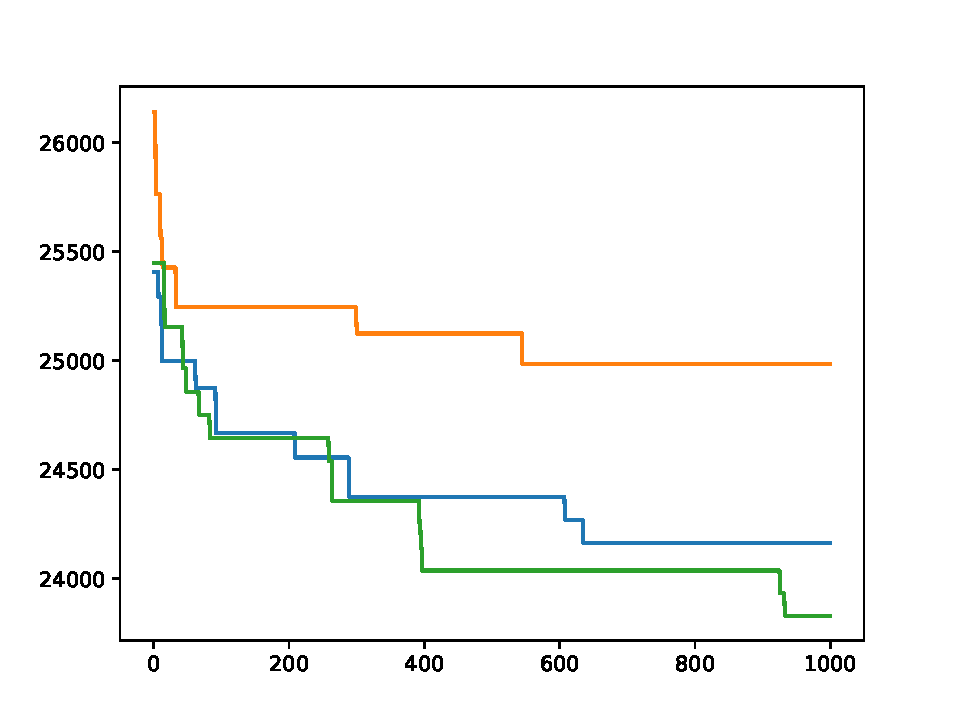
\includegraphics[scale=.5]{../Plots/5,2,Threshold-100,mutcrossmult.pdf}
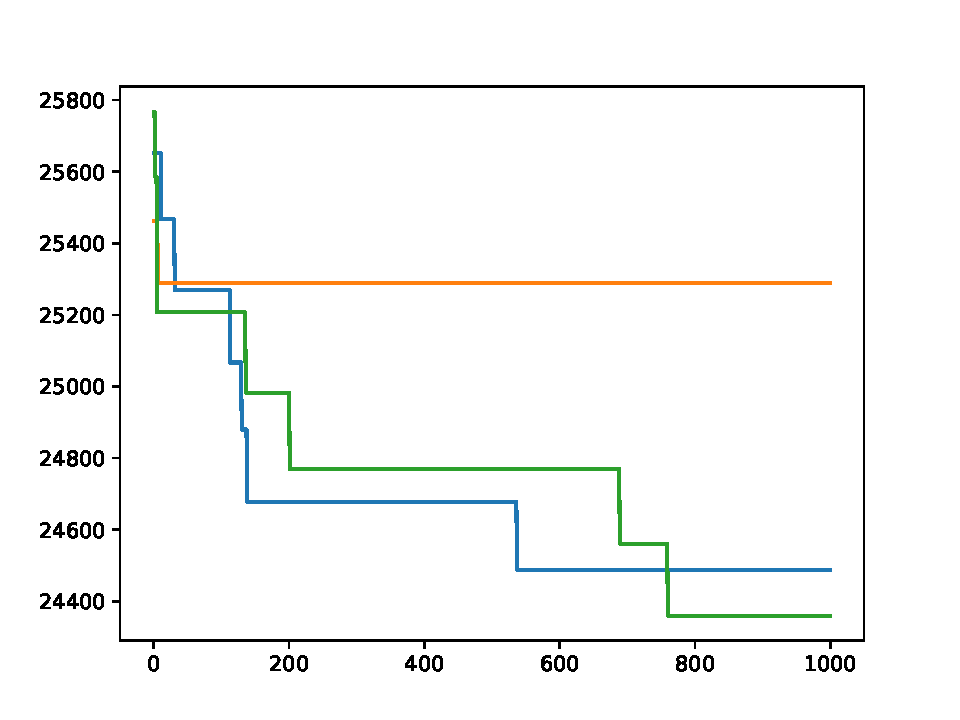
\includegraphics[scale=.5]{../Plots/new/5,2,mutcmul,threshold-150.pdf}
\caption{Comparaison for $\lambda = 5$, $\mu = 2$ and threshold selection with
constant parameter $T = -150$ of mutation variation (in blue), crossover
variation (in orange) and another variation consisting of a mix of both (in
green).}
\label{Thresholdcomparevariation}
\end{figure}
\end{frame}

\begin{frame}
	Threshold selection with $T = -80$.
\begin{figure}
\centering
%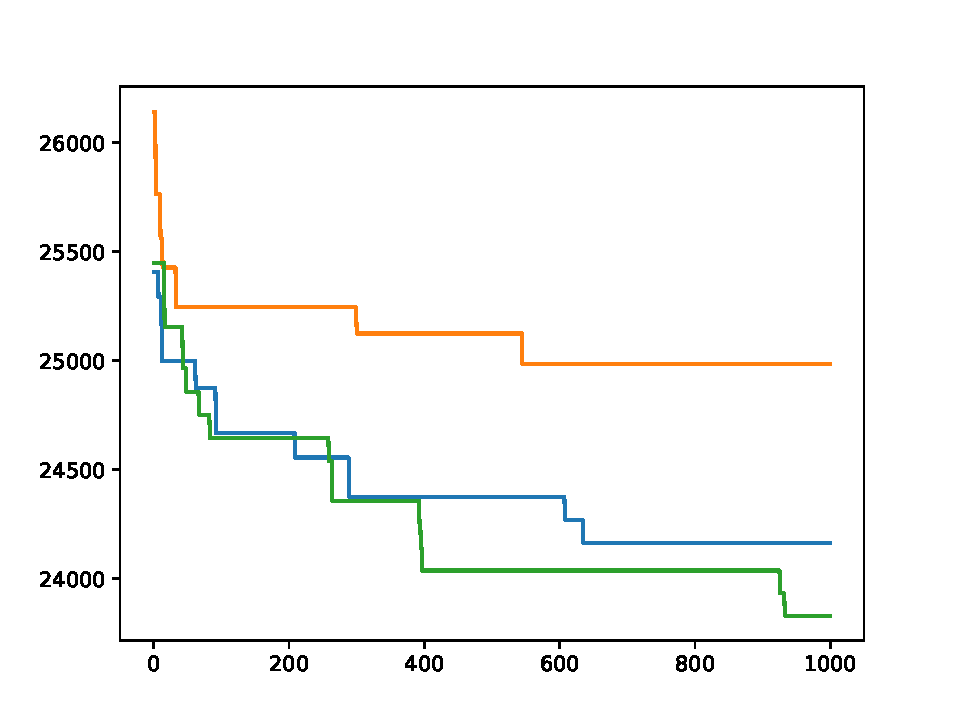
\includegraphics[scale=.5]{../Plots/5,2,Threshold-100,mutcrossmult.pdf}
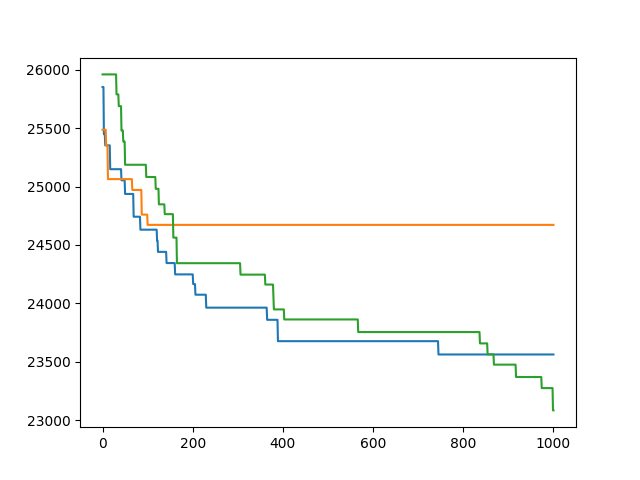
\includegraphics[scale=.5]{../Plots/new/5,2,mutcmul,Threshold-80.png}
\caption{Comparaison for $\lambda = 5$, $\mu = 2$ and threshold selection with
constant parameter $T = -80$ of mutation variation (in blue), crossover
variation (in orange) and another variation consisting of a mix of both (in
green).}
\label{Threshold-80comparevariation}
\end{figure}
\end{frame}

\begin{frame}
	Final heuristic.
\begin{figure}
\centering
%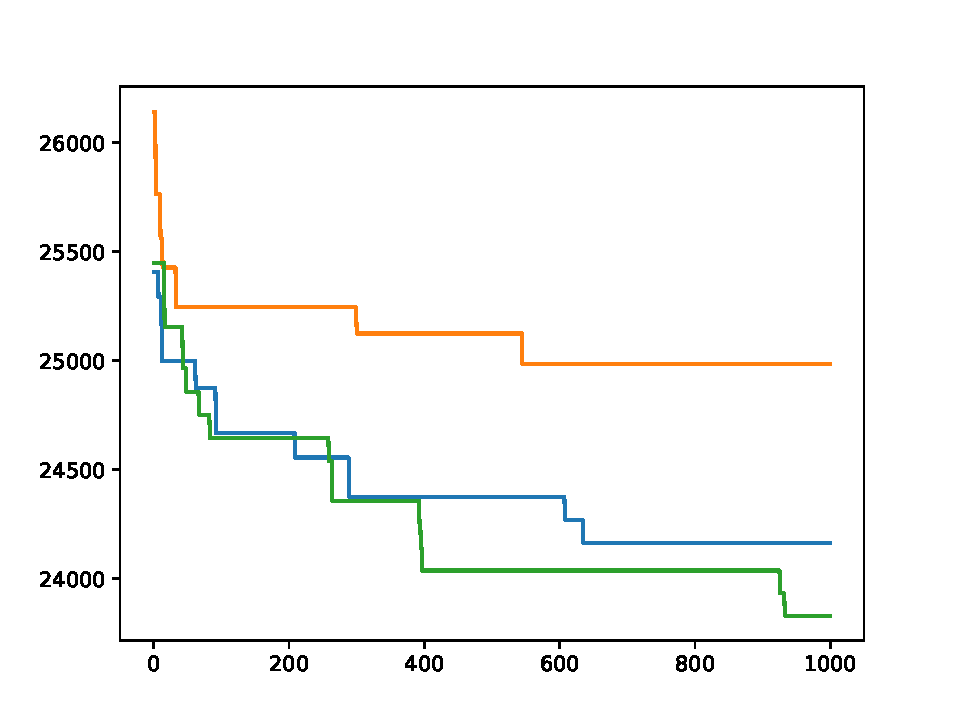
\includegraphics[scale=.5]{../Plots/5,2,Threshold-100,mutcrossmult.pdf}
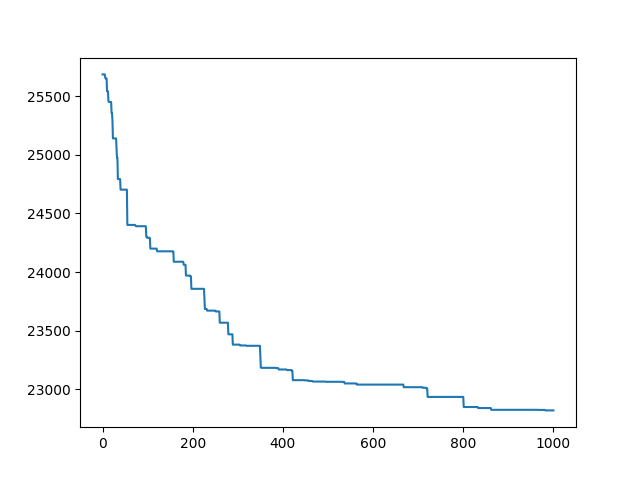
\includegraphics[scale=.5]{../Plots/new/11,3,mut,Boltzmann.png}
\caption{Comparaison for $\lambda = 11$, $\mu = 3$ and Boltzmann selection with
constant parameter $T = 1000$ and mutation variation (in blue)}
\label{MutationBoltzmann}
\end{figure}
\end{frame}

\end{document}
